\section{Diodo 1N4007: caratteristica volt-amperometrica}

\begin{wrapfigure}[22]{r}[0pt]{130mm}
	\caption{ciao}
	\label{fig:diodo}
	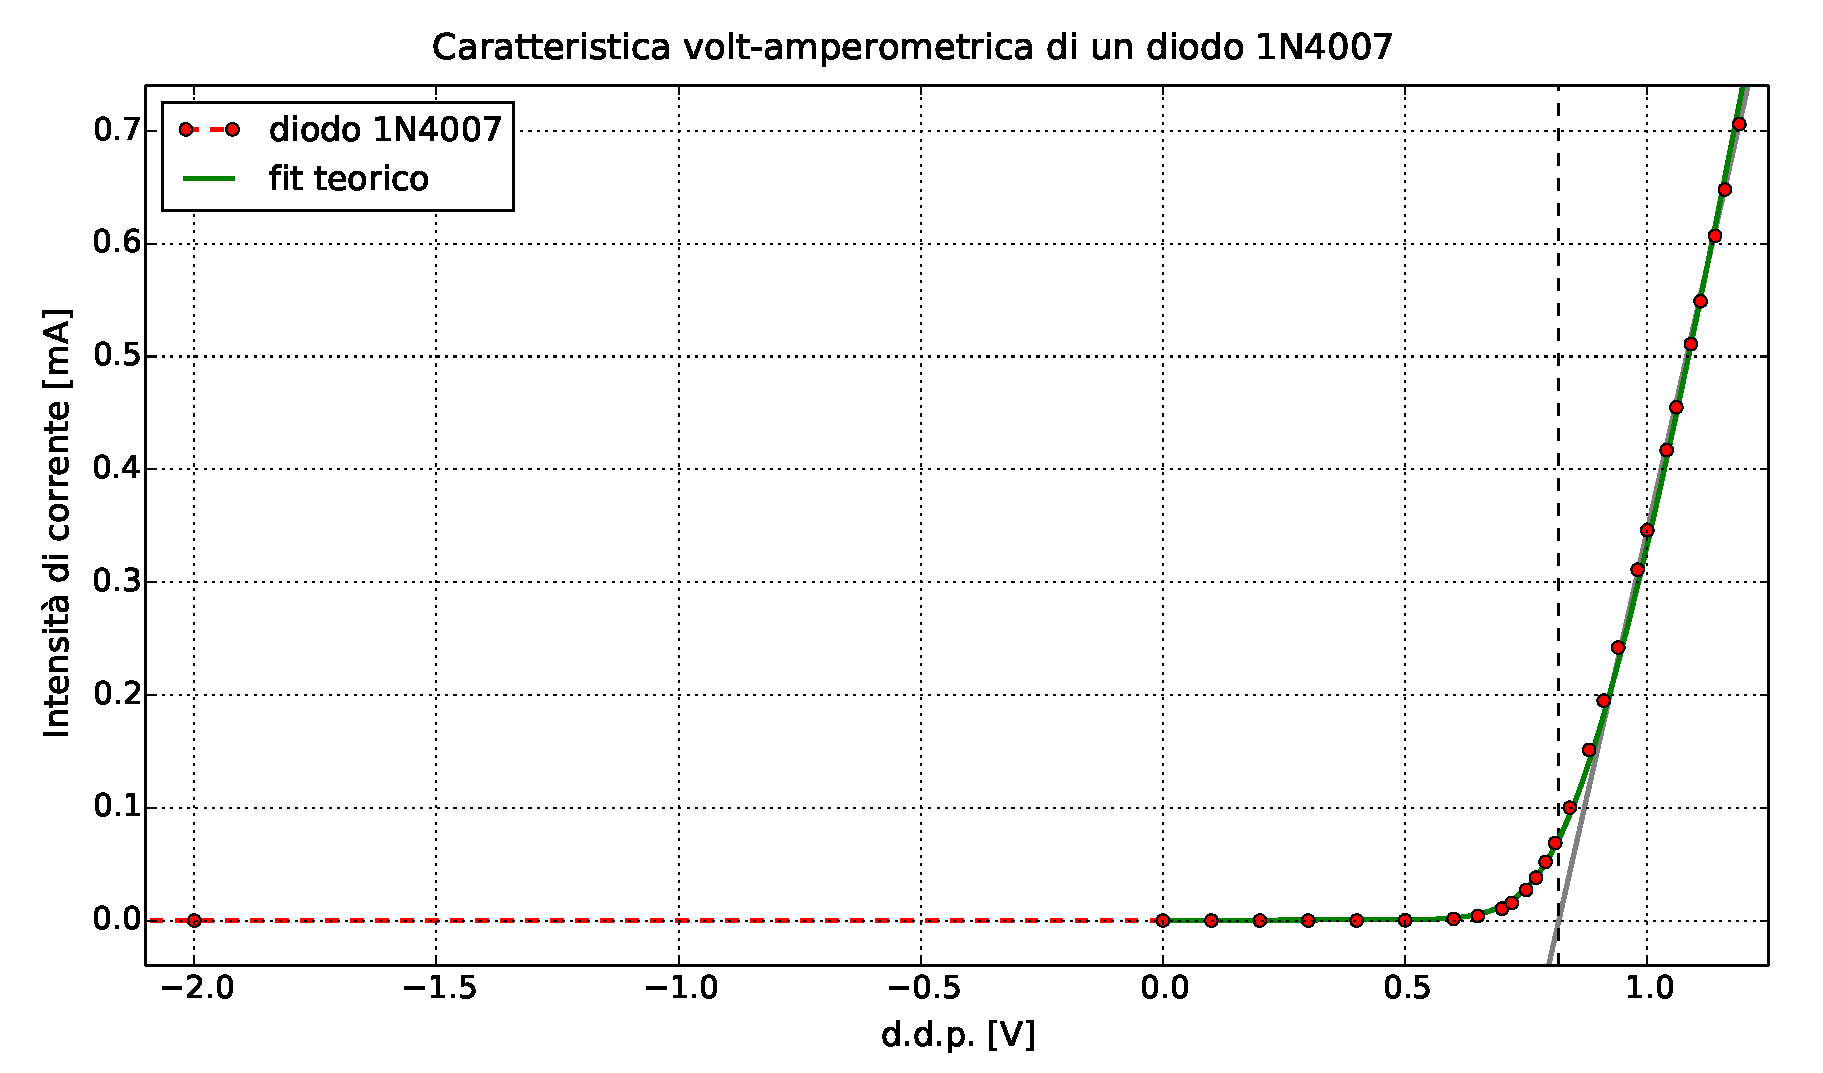
\includegraphics[width=0.75\textwidth]{diodo.pdf}
\end{wrapfigure}

Per studiare la caratteristica volt-amperometrica del diodo abbiamo dovuto separare l'analisi in due fasi distinte: una prima fase in cui abbiamo analizzato il comportamento del diodo polarizzato in diretta e una seconda fase in cui ne abbiamo analizzato il comportamento in inversa.
Utilizzando la breadboard come support,o abbiamo creato un circuito composto dal genertore di tensione continua (max $\pm \SI{25}{\volt}$), il diodo e il multimetro digitale in modalità amperometro. Aumentando progressivamente la tensione, abbiamo letto sull'amperometro i valori della corrente che attraversava il circuito.
Facendo attenzione che la corrente non superasse il valore di \SI{700}{\milli\ampere} abbiamo quindi popolato l'asse positivo del grafico. In seguito abbiamo girato il diodo in modo che fosse alimentato in inversa e abbiamo popolato anche l'asse negativo del grafico, ottenendo la caratteristica volt-amperometrica completa del diodo. Il risultato è esposto in Figura \ref{fig:diodo}.
\\
\\
Dal grafico osserviamo che i dati ricavati seguono la legge teorica, la cui formula è:
\begin{equation}
I_{D} \, = \, I_{S} \left( e^{\frac{q V_d}{nKT}} -1 \right)
\label{eq:diode}
\end{equation}

\section{Cella solare: caratteristica volt-amperometrica}
\subsection{cella solare al buio}

\begin{equation}
FF \, = \, \frac{I_{@P_{max}} \,\, V_{@P_{max}}}{I_{sc} \,\, V_{oc}}
\label{eq:FF}
\end{equation}

\subsection{cella solare alla luce}


\section{ponte di Graetz}